% Compile with pdfLaTeX (or Tectonic) from this folder. Keep assets/ alongside this file.
% Original time-series screenshots are extracted directly from the supplied PDF.
% US Letter, one page. Editorial changes are documented in the companion log.
\documentclass[10pt,letterpaper]{article}
\usepackage[T1]{fontenc}
\usepackage{lmodern}
\usepackage[margin=0.45in]{geometry}
\usepackage{microtype}
\usepackage{booktabs,tabularx,array}
\usepackage{xcolor}
\usepackage{graphicx}
\graphicspath{{assets/}}
\usepackage{enumitem}
\usepackage{titlesec}
\definecolor{navy}{HTML}{18364A}
\definecolor{muted}{HTML}{52606B}
\pagestyle{empty}
\setlength{\parindent}{0pt}
\setlength{\parskip}{4pt}
\AtBeginDocument{\fontsize{9.5}{11.2}\selectfont}
\titleformat{\section}{\fontsize{11}{12.5}\selectfont\bfseries\color{navy}}{}{0pt}{}
\titlespacing*{\section}{0pt}{7pt}{3pt}
\setlist[itemize]{leftmargin=12pt,itemsep=1pt,topsep=2pt,parsep=0pt}
\newcolumntype{L}{>{\raggedright\arraybackslash}X}
\begin{document}
{\LARGE\bfseries\color{navy} Santa Clara Market Overview}\par
\vspace{6pt}
{\color{navy}\hrule height 0.8pt}

\vspace{7pt}
\begin{minipage}[t]{0.455\textwidth}
\vspace{0pt}
\setlength{\parskip}{4pt}
\section*{Market Overview \& Pricing Trends}
Median closing prices follow a seasonal pattern, generally lowest in winter and highest in spring. Average days on market show the reverse pattern: longest in winter and shortest in spring. However, average days on market increased in 2025 and again in 2026, possibly signaling weaker housing demand. This pattern may help explain the subtle decline in annual peak and low closing prices in 2025 and 2026.

\section*{Market Activity}
Closing prices relative to original listing prices have trended downward since their April 2024 peak. By July 2025, homes were closing at approximately their original listing prices. This trend continued into 2026, with homes selling for less relative to original asking prices than in 2024 and 2025.

After peaking in May 2024, closed sales reached their low in January 2026, then gradually recovered, doubling to a 2026 peak of \textbf{528 in June}. Monthly new listings remained relatively similar, peaking in May in 2024, 2025, and 2026. The wider gap between incoming supply and completed sales suggests more choice for buyers and greater competition among sellers.

\section*{Competitive Landscape}
\textbf{Andy Tse} leads individual agents by a wide margin in both properties sold and sales volume. David Lillo, Xiaozhu Kang, and Sophie Shen rank second through fourth in both measures; each sold over 80 more properties than the fifth-ranked agent by properties sold. \textbf{Compass, Coldwell Banker Realty, and Intero Real Estate Services} hold the top three office positions in both measures. Concentration among leading agents and offices suggests that listing access, brand reach, and productivity remain important competitive advantages.

\end{minipage}\hfill
\begin{minipage}[t]{0.52\textwidth}
\vspace{0pt}
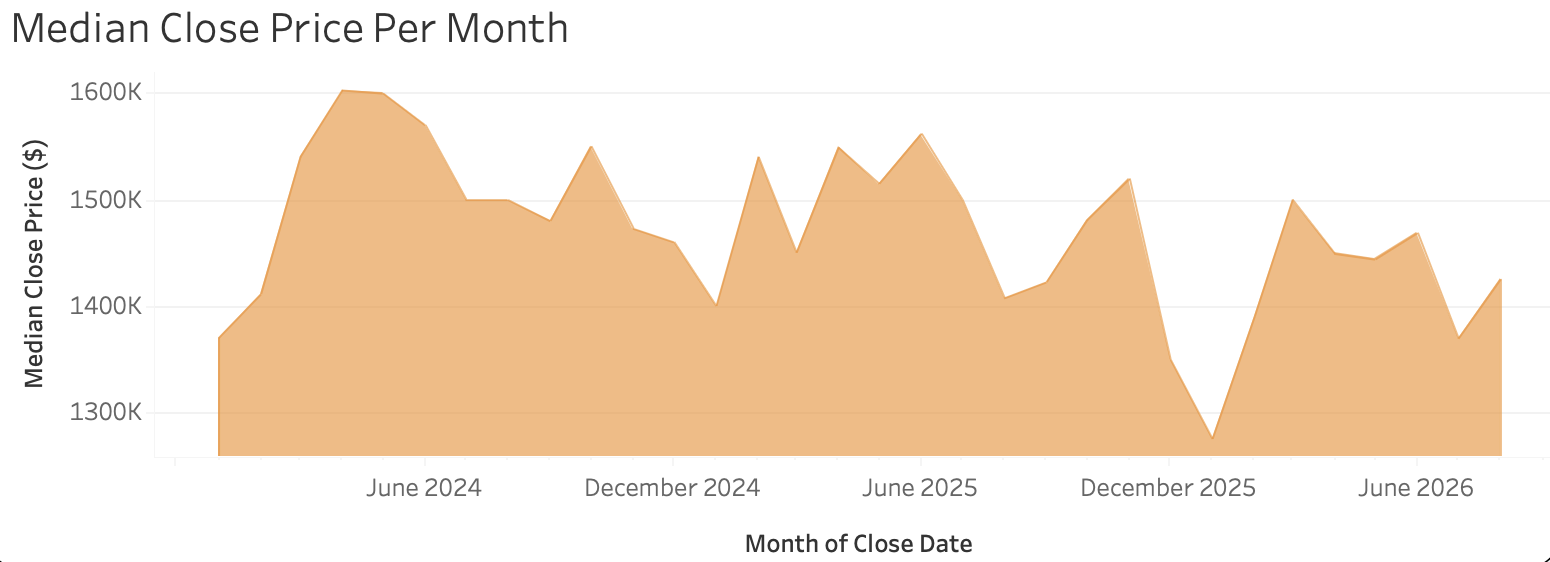
\includegraphics[width=\linewidth]{median-close-price.png}\par\vspace{5pt}
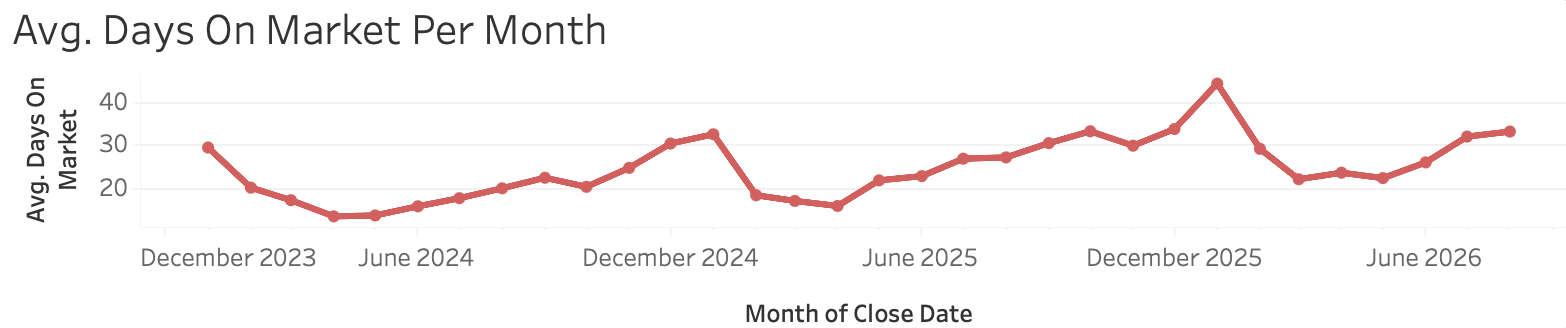
\includegraphics[width=\linewidth]{average-days-on-market.png}\par\vspace{5pt}
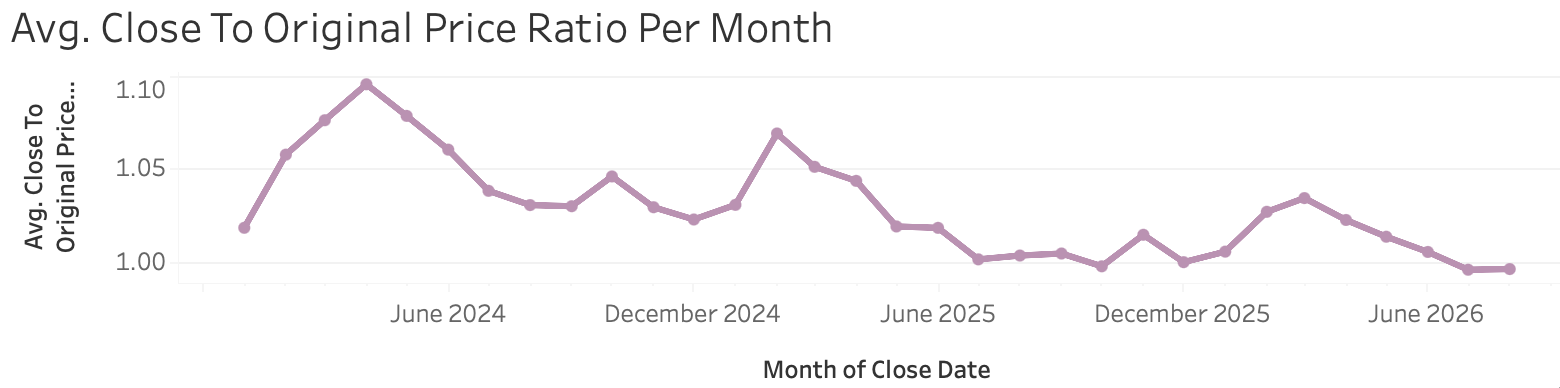
\includegraphics[width=\linewidth]{close-to-original-price-ratio.png}\par\vspace{5pt}
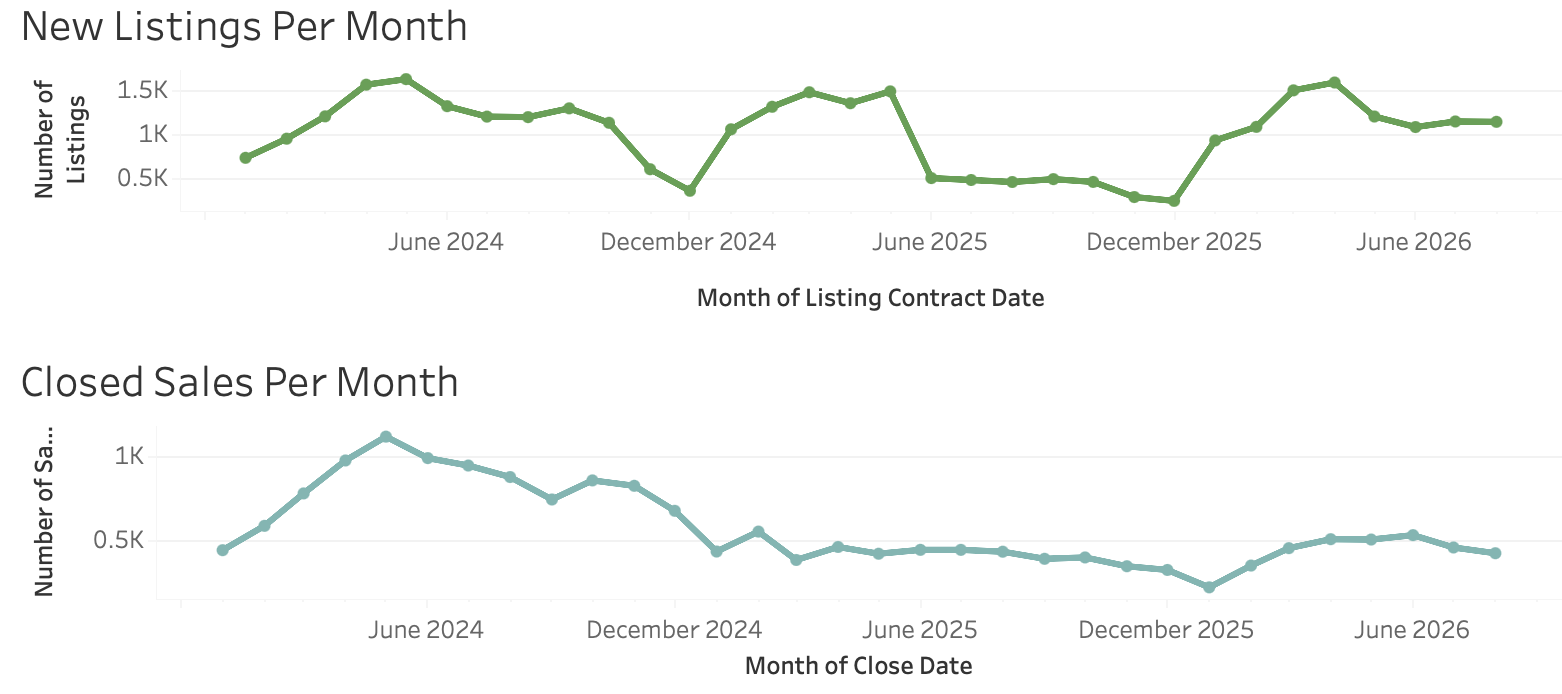
\includegraphics[width=\linewidth]{new-listings-and-closed-sales.png}
\end{minipage}

\vspace{3pt}
\begin{minipage}[t]{0.485\textwidth}
{\small\bfseries\color{navy} Listing agents}\par\vspace{1pt}
\fontsize{9}{10.5}\selectfont
\setlength{\tabcolsep}{3pt}
\begin{tabularx}{\linewidth}{@{}Lrr@{}}
\toprule
\textbf{Agent} & \textbf{Sold} & \textbf{Volume (\$)}\\
\midrule
Andy Tse & 173 & 390,988,376\\
David Lillo & 152 & 298,583,259\\
Xiaozhu Kang & 142 & 226,485,384\\
Sophie Shen & 133 & 174,835,385\\
Bernadina Romero & 52 & ---\\
Suzie Gibbons & 48 & ---\\
Bonafede Team & --- & 137,150,985\\
Kevin Swartz & --- & 132,743,011\\
\bottomrule
\end{tabularx}
\end{minipage}\hfill
\begin{minipage}[t]{0.495\textwidth}
{\small\bfseries\color{navy} Listing offices}\par\vspace{1pt}
\fontsize{9}{10.5}\selectfont
\setlength{\tabcolsep}{3pt}
\begin{tabularx}{\linewidth}{@{}Lrr@{}}
\toprule
\textbf{Office} & \textbf{Sold} & \textbf{Volume (\$)}\\
\midrule
Compass & 2,630 & 4,388,276,833\\
Coldwell Banker Realty & 2,410 & 3,967,504,475\\
Intero Real Estate Services & 2,402 & 3,958,746,763\\
Christie's International R\ldots & 958 & 1,631,236,998\\
Kw Bay Area Estates & 518 & 871,668,561\\
Exp Realty Of California Inc & 267 & ---\\
Keller Williams Realty-Sili\ldots & --- & 643,552,618\\
\bottomrule
\end{tabularx}
\end{minipage}

{\fontsize{8}{9.5}\selectfont\color{muted}
Tables retain all entries and exact values shown in the source ranking charts. ``---'' means not shown in the corresponding chart, not zero. Truncated office names are retained from the source.\par}

\vfill
\section*{Key Takeaways}
\begin{itemize}
\item Prices and days on market remain seasonal, with lower closing prices and longer selling times year over year.
\item Since July 2025, buyers have purchased homes at approximately original listing prices.
\item Softer demand and similar incoming listing levels suggest a wider selection for buyers.
\item Andy Tse, David Lillo, Xiaozhu Kang, and Sophie Shen dominate agent sales counts and volume.
\end{itemize}
\vspace{5pt}
{\fontsize{8}{9.5}\selectfont\color{muted}
Source: \textit{Santa Clara Market Overview-2.pdf}, pp.~1--4. Original time-series screenshots retained; narrative condensed; rankings set as LaTeX tables.\par}
\end{document}
